\documentclass[12pt]{report}
\usepackage{pdfpages}
%\usepackage{amsmath}
\usepackage{enumitem}

\begin{document}
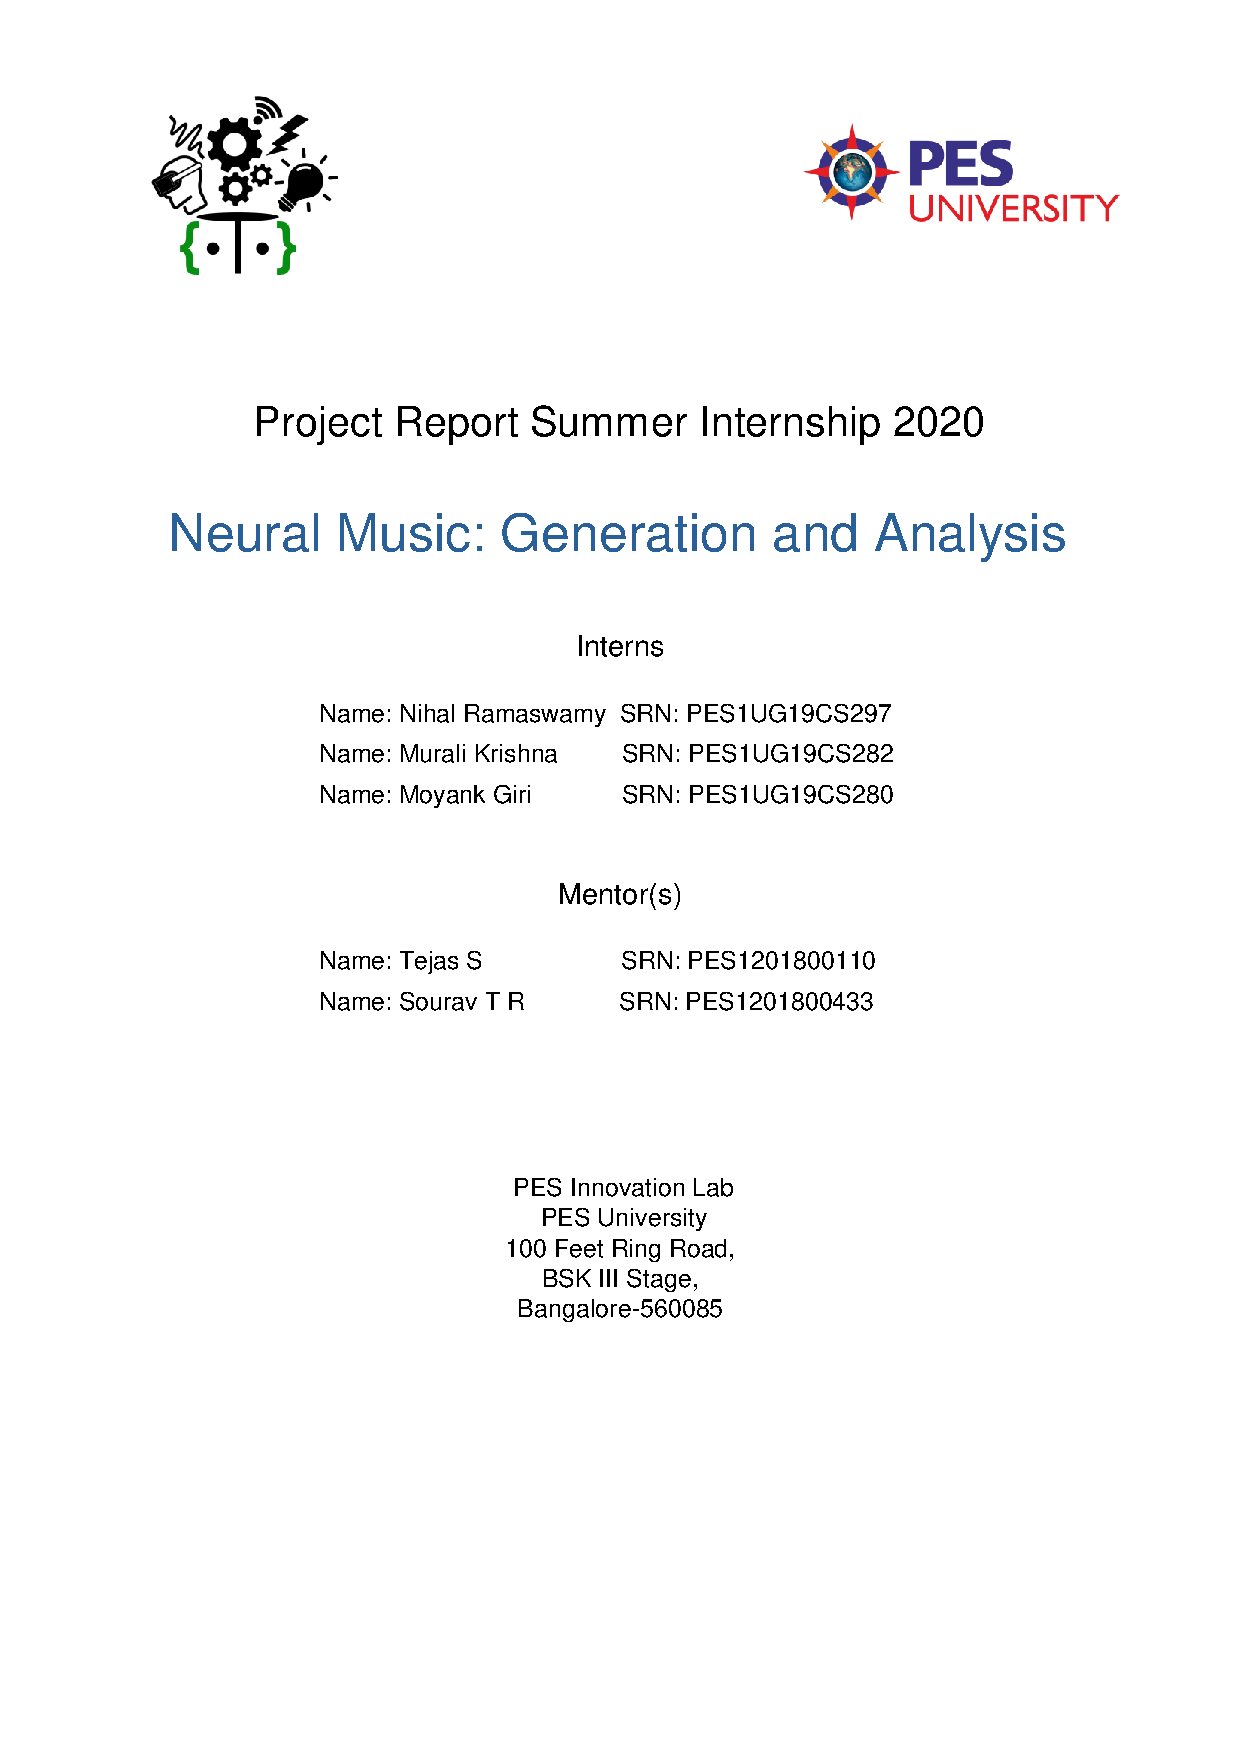
\includepdf[pages={1}]{coverpage.pdf} 

\begin{abstract}
Music composition, by its very nature, is a dynamic process. It is regarded as an art form, an expression of the very essence of what it is to be human. Music has been around from time immemorial, and has undergone a continuous process of evolution to reach the form  we consume in mainstream media today. Most composers would attest to the challenges involved in creating a piece of music that sounds satisfactory. It might not be entirely possible to automate the entire process of music composition. Recent advances in technology, however, allow machines to contribute to this process in an assistive capacity. In its basic form, a song can be split into a lead track, and a backing track. The lead track usually forms the backbone of the song and gives the latter its distinctive feel; however, it is usually incomplete without a corresponding backing track (also called an Accompaniment). While technologies exist that create contextual music, the aim of this project is to create a model that can specifically generate a backing track for an input lead track, or generate a lead track for an input backing track. The approach used involves a combination of an RNN-LSTM machine learning model, and algorithmic analysis of the music itself. The input music is first passed through a Noise Cancellation Engine to ensure accurate results, after which tonal analysis of the music is carried out. Finally, the results are fed into the model which then returns the output.

\end{abstract}

\tableofcontents
%\listoffigures
%\listoftables

\chapter{Introduction}
\textbf{What?}\\
A web application that allows a musically-inclined user to generate contextual music and edit the results via a graphical user interface.\\
Domains:
\begin{itemize}
  \item Web Development
  \item Deep Learning
  \item Algorithms
\end{itemize}
\textbf{Why?}\\
The process of composing a lead to an existing accompaniment, or composing an accompaniment to an existing lead, can be a daunting process. Neural Moosic aims to automate either process, allowing musicians to focus on the aspect they are better at.\\ 
\textbf{How?}\\
The approaches for both processes are different. Both use an RNN-LSTM deep learning model, however, in different capacities. The process of Accompaniment generation is primarily algorithmic; Tonal analysis is conducted on the lead, and suitable chords are generated, and are then fed to the model to provide varied results. The process of Lead generation is primarily via the Deep Learning model, with initial algorithmic analyses.\\
\textbf{Who?}\\
Neural Moosic is primarily for musicians who are good at only one of the above mentioned aspects of composition; Lead, or Accompaniment. It allows for a well rounded composition to be made. However, amateur musicians may also find the project useful, to experiment with different types of sounds.

\section{Problem Statement}
To help musicians improve the audio-quality of their song, generate a backing track for their lead and vice-versa to help kick start a composition with a piece of music generated by our deep-learning model, via a user-friendly web application.

\chapter{Literature Survey/Related Work} 
The solutions to generate lead music tend to involve the use of sequential deep learning models.\\In a paper titled ``Music Generation by Deep Learning– Challenges and Directions`` authored by Jean-Pierre Briot and Francois Pachet, they detail their process of generating music using RNN-LSTMs on multiple datasets using GPUs to help accelerate the training process. The aim is to extend this approach to specific scales and chords. \\Approaches to backing track generation tend to use proprietary algorithms. \\Popular noise cancellation methods usually involve algorithms for Active noise cancellation, or Source Separation. The theory behind the former is taken up from day to day usage of cellphones; Most cellphones in recent times have two microphones, where one microphone records the noise and the other microphone records the audio from which noise needs to be removed.
\chapter{Solution Architecture}
\section{Overview}
In this section, a brief overview of the processes involved in the generation of a Backing Track is provided. This can be thought of as a two part process: Processing of user-input, and Tonal analysis of the processed input. 

\begin{figure}[ht]
  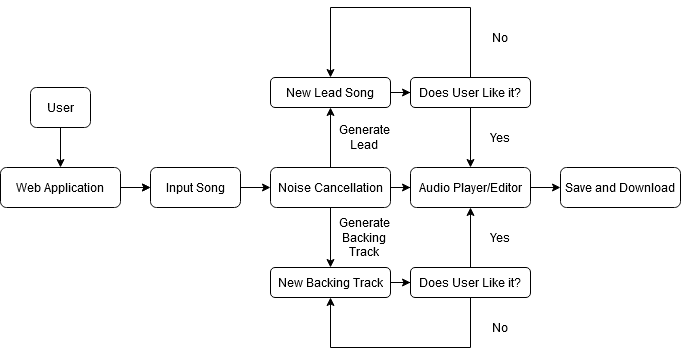
\includegraphics[width =\columnwidth]{FlowChart_overall.png}
  \caption{Flowchart of how app works}
  \label{flowchart_overall}
\end{figure}


\section{Noise Cancellation and Source Separation}
%In this, we have made a folder containing all the common noises that we can find in our surroundings. This model runs the input song and tries to see if there were any matching songs. If the model detects any matching song, that part of the song is removed.
The project accomplishes noise cancellation by using the concept of active noise cancellation.\\
The active noise cancellation used for this project requires that two inputs are provided, i.e. the noise that has to be removed, and the audio file from which the noise has to be removed. Hence for the above mentioned inputs, a dataset which contains various noise files which are common in everybody's day to day life is employed.\\The current idea of the model is that it would parse all the various sounds mentioned in the noise folder and try to remove all those noises from the given audio file so that the noise from the audio file provided can be minimized.\\
The steps included for the noise cancellation algorithm are: 
\begin{enumerate}[leftmargin = 2cm]
\item An FFT is calculated over the noise audio clip
Statistics are calculated over FFT of the the noise (in frequency)
\item A threshold is calculated based upon the statistics of the noise (and the desired sensitivity of the algorithm)
\item An FFT is calculated over the signal
\item A mask is determined by comparing the signal FFT to the threshold
\item The mask is smoothed with a filter over frequency and time
\item The mask is appled to the FFT of the signal, and is inverted
\end{enumerate}
The project also uses a blind source separation code in order to have a better result in separation of the noise and having any kind of noises in the audio file provided.
\begin{figure}[ht]
  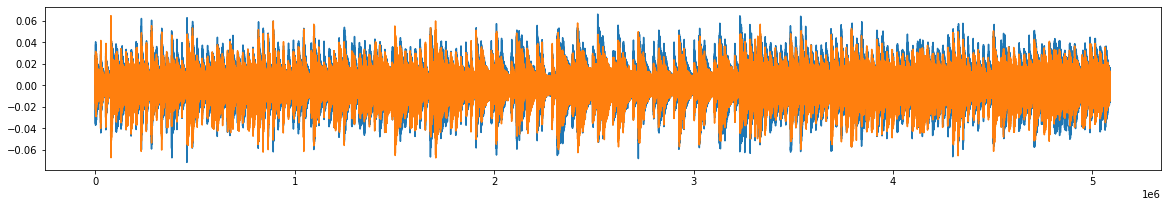
\includegraphics[width =\columnwidth]{noise_audio.png}
  \caption{audio file with noise}
  \label{song_with_noise}
\end{figure}
\begin{figure}[ht]
  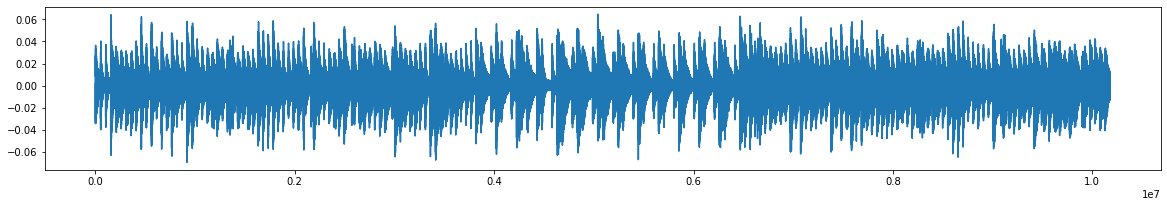
\includegraphics[width =\columnwidth]{noiseless_audio.png}
  \caption{audio file after noise cancellation}
  \label{song_without_noise}
\end{figure}
\section{Input and Pre-processing}
The noise cancelled input file is still in the mp3/wav format. However, this format is gibberish to the computer, as typical audiofile formats are, in essence, waveforms. This means that there is no 'note' attached intrinsically to those frequencies. This is a major hurdle, as any sort of predection/generation fundamentally requires a knowledge of the notes present in the song. This information is provided by the MIDI format (Musical Instrument Digital Interface).\\The MIDI format is very different, in that it does not store actual audio waveforms; This means that only necessary information is kept, and in a machine-readable manner. The caveat here is that MIDI files are almost exclusively generated from scratch; this is what allows for pure audio-quality and zero noise. Hence, to obtain a viable MIDI file, we must perform a two-fold process: Meloldy Extraction and Note Quantization. Melody extraction is the task of automatically estimating the fundamental frequency corresponding to the pitch of the predominant melodic line of a piece of polyphonic (or homophonic) music. It is also called F0 Estimation. Melody extraction is, in essence:
\begin{enumerate}[leftmargin=2cm]
\item Estimating when the melody is present and when it is not (also referred to as voicing detection).
\item Estimating the correct pitch of the melody when it is present.
\end{enumerate} Once the pitch contour of the melody is extracted, the next step is to segment it into notes and quantize the pitch of each note, producing a discrete series of notes that can then be exported into a MIDI format. Quantizing a continuous pitch sequence into a series of notes is an active area of research and remains and open problem. Still, fairly decent results may be obtained using a series of heuristics: \begin{enumerate}[leftmargin=2cm]
\item Convert the pitch sequence from Hertz to (fractional) MIDI note numbers.
\item Round each value to the nearest integer MIDI note number.
\item Iterate over the sequence and whenever the pitch changes start a new note.
\end{enumerate}

\section{Model}
\subsection{Model Specifications}
The model is an RNN-LSTM model written in Tensorflow and is trained using CUDA.\\
The model has 3 layers; each layer has 512 hidden layers with a dropout rate of 0.4 and a batch size of 128.\\
The model was run for a total of 200 epochs.
\\However, these numbers can be tweaked for different results.
\subsection{Training the Model}
Initially, the dataset is split by the Scale of the songs. The model is then trained for each of those scales, and the best weights for that particular scale are saved; This eliminates redundancy in retraining the model every time a new song is generated.
\begin{figure}[ht]
  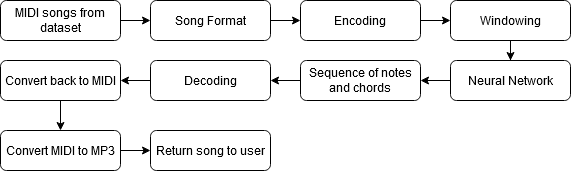
\includegraphics[width =\columnwidth]{Flowchart_model.png}
  \caption{Flowchart of model}
  \label{flowchart_model}
\end{figure}

\section{Track Generation}
\subsection{Generating Backing Track}
Initially, a list of all possible chords for the song's scale is made, by extracting the song-scale data from the MIDI file. The file is then segmented using its Time signature.
Iterating over each obtained sub-segment, a set of viable chords for the segment in question is obtained. This is done by intersecting the notes in the segment with each possible chord, and choosing the chord with the highest intersection. The list of chords obtained is then passed through the Deep Learning Model, and a list of 'mini-songs' are obtained. These are finally recombined to produce the backing track.

\chapter{Results and Discussion}
As we approach the end of the first phase of this internship, Neural Moosic, in its current state, is capable of generating an appropriate backing track given an input lead track. It does so with a fair degree of accuracy, despite the model still being somewhat rudimentary. As improvements are made to the model, we expect even better results. Figure 4.1 is a screenshot of a backing track generated for an excerpt of the song 'Jingle Bells'.
\begin{figure}[ht]
  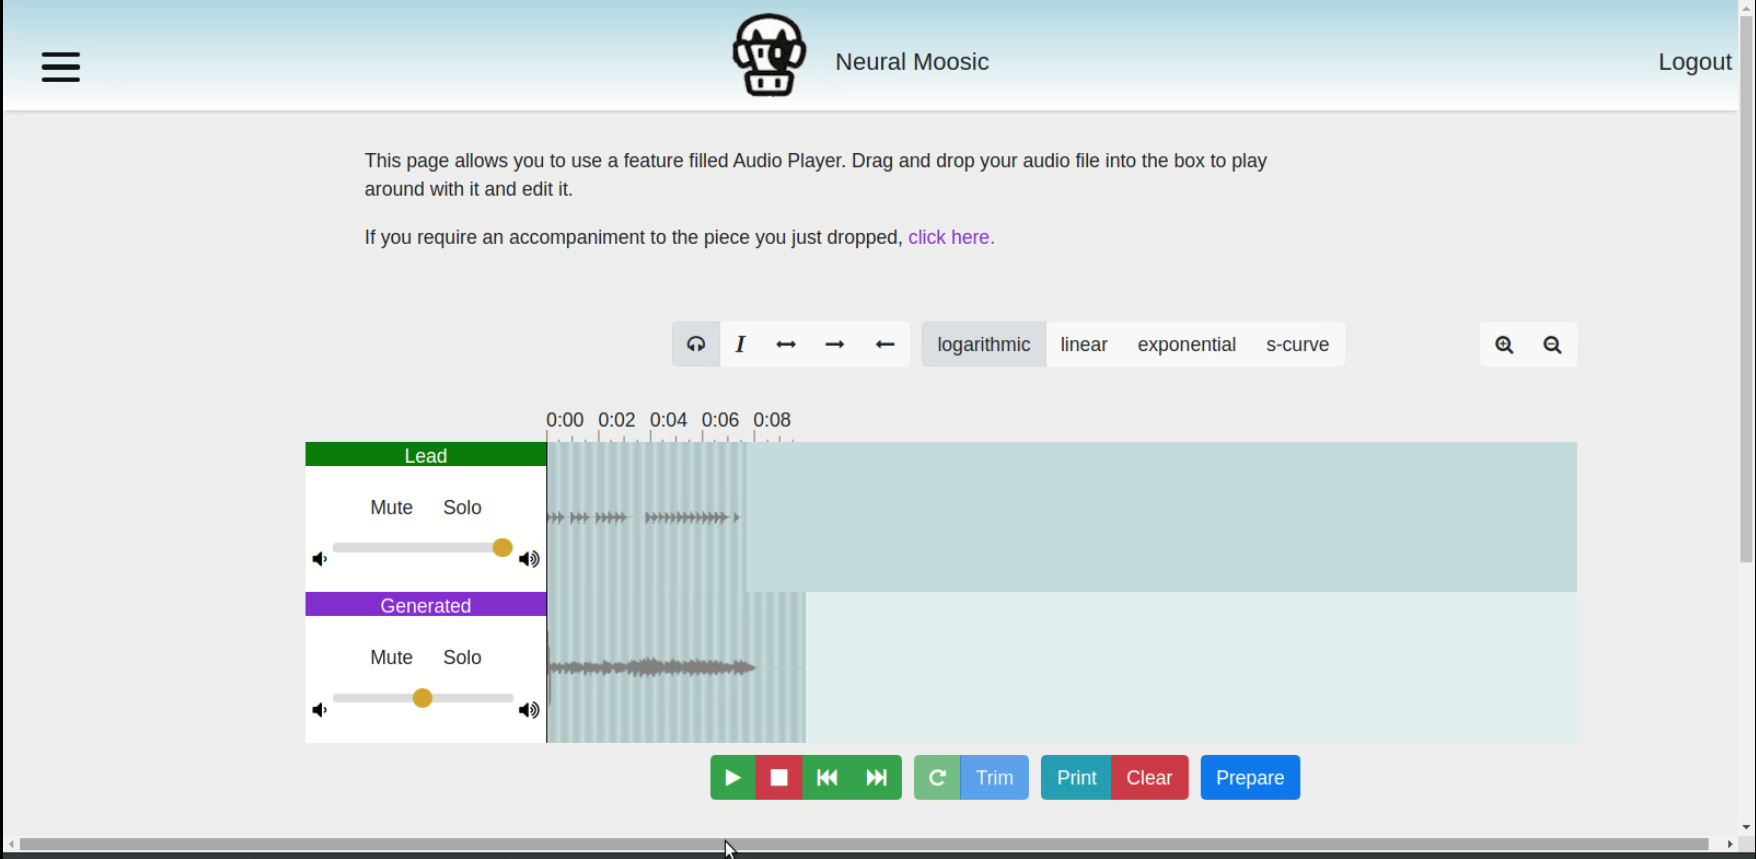
\includegraphics[width =\columnwidth]{sc.png}
  \caption{Backing track generated for Jingle Bells}
  \label{working demo}
\end{figure}

\chapter{Hardware and Software Requirements}
The client side requirement is a Javascript-enabled browser, preferably Google Chrome or Mozilla Firefox. 
On the server side, ReactJs 16.3.1 and Flask 1.1.2 were used in the architecture of the web-app; The training of the deep-learning model necessitated the use of Tensorflow 2.2.0 and the NVIDIA CUDA kit 10.1, to allow for training on GPU. The said GPU was an NVIDIA GeForce 1650x. To extract data from the MIDI files, the python library music21 was used.

\chapter{Conclusions and Future Work}
There is still scope for improvement, with plans for more chords, smoother transitions as well as a more dynamic pattern generation in the pipeline. The goal is also to finish the Lead track generation model, which is right now in progress; This will be achieved with a greater focus on the Deep Learning model. The focus will also shift to analysis of music, and its applications.
%Please make sure you keep a log of all the resources you have used. This includes websites, tutorials, videos, papers or even blogs can be cited.

\bibliographystyle{ieeetr} 
\bibliography{bibliography}
\cite{wiki:latex}
\cite{wiki:fermat}
\cite{DBLP}
\cite{huang}
\cite{pitch}
\cite{6155601}
\cite{1561271}
\cite{bogdanov:Essentia:ISMIR13}

% \appendix 
% \chapter{sample appendix header 1}
% %\label{app_1}
% Appendices: 
% Proofs, links to your code and any other misc. info that doesn?t fit in nicely into other sections. 


\end{document}
